\begin{figure}[htb]
  \begin{center}
    \resizebox{\textwidth}{!}{
      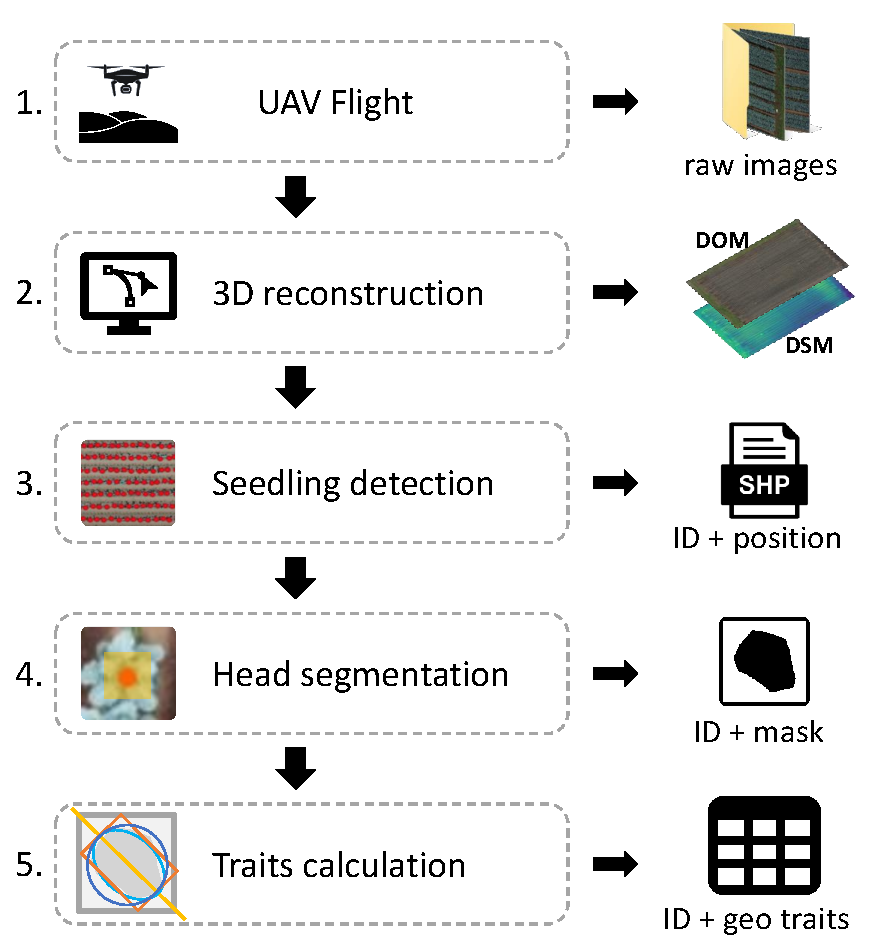
\includegraphics{figures/bro/Fig.4_general_workflow.pdf}
    }
  \end{center}
  \caption[Workflow and schematic of the study method]{
    Workflow and schematic of the study method. First was the UAV-based pipeline which was used to obtain the time-series head size information (geometry traits) of all broccoli heads during the growing season (the outputs of each step are the inputs of the next step). We then obtained a simple growth model between head size and temperature data, which was combined with price data obtained via a market survey to build the profit prediction model for the optimal harvest date.
  }
  \label{fig:bro4}
\end{figure}